\chapter{Implementación}


% Más subsecciones dependiendo de la metodología empleada


% Debe ser la sección más larga del documento.
% Usar herramientas de Ingeniería: diagramas, esquemas, plantillas, etc.

% - Incluir un diagrama de la arquitectura del sistema (visión general).
% - Indicar qué herramientas de la sección anterior se eligen para el
% desarrollo, por qué y para qué.
% - Poner solo pequeños trozos de código si es necesario para explicar
% detalles de implementación o justificar decisiones del diseño o de la
% tecnología.

\section{Exploración de funcionalidades}
% https://github.com/daniharo/mi-banda-bot

\subsection{Infraestructura de contenedores}

% docker, docker-compose

\subsection{Conexión a base de datos}


\subsection{Manejo de mensajes de Telegram}


\section{Internacionalización}


\section{Plantillas: separación MVC}


\section{Unirse a un grupo}


\section{Crear, mostrar y eliminar agrupaciones}



\section{Optimización de la autenticación en cada mensaje}

% middleware: useAccount


\section{Crear, mostrar y eliminar eventos}


\subsection{Selector de fecha}


\subsection{Guardar sesión en la base de datos}

% qué se guarda en la sesión: id de usuario, paso dentro de una conversación, etc

% contribución a grammY

% problema: tests


\section{Configuración del \textit{linter}}

% ESLint, ESLint-typescript


\section{Limitación de errores para el bot}\label{section:errorBoundary}
% Global error boundary


\section{Mejora del flujo de trabajo para depurar}
% node inspect (commit https://github.com/daniharo/mordente/commit/5a64a8516519d1f21e33a8810252bb9b79a3588b)


\section{Respuestas de asistencia prevista}
% https://github.com/daniharo/mordente/commit/9d2059609cc696405f6f4cbd2b2590ff2878eb98


\subsection{Pedir justificación}
% https://github.com/daniharo/mordente/commit/06efba49a35e562bf23756bc2fa2fdf8d150ca47

\subsection{Notificar administradores}
% https://github.com/daniharo/mordente/commit/fb7e33e4d485841c9d14a15acff932f66f270476

\section{Asignación de miembros a eventos}
% https://github.com/daniharo/mordente/commit/9e951c77ee1b2a68ad6096b7ebf269192ff75522

% https://github.com/daniharo/mordente/commit/77ad84b13aae9dba6c6f44f890fb200695459148
% https://github.com/daniharo/mordente/commit/b111f68ee919500346a61c1c3d711caed6fd9c17
Ahora haremos que los eventos puedan ser asignados a usuarios concretos.

Durante la creación de un evento, preguntaremos a un usuario si quiere asignarlo a todos los usuarios o si asignará manualmente más tarde\footnote{\textit{Commit:} \url{https://github.com/daniharo/mordente/commit/9e951c77}}. Haremos también que los usuarios solo puedan ver los eventos que tienen asignados\footnote{\textit{Commit:} \url{https://github.com/daniharo/mordente/commit/77ad84b1}}. Por último, implementaremos un menú paginado que permita a los administradores elegir exactamente qué miembros estarán asignados a cada evento\footnote{\textit{Commit:} \url{https://github.com/daniharo/mordente/commit/b111f68e}}.

\section{Recordatorio de eventos diarios}
% https://github.com/daniharo/mordente/commit/33859f0544f298262d72be75aac76bdbc1244d31

La historia de usuario relativa a los recordatorios diarios de eventos es la única que no dispara una petición al bot sino que dispara el bot por sí mismo cada cierto tiempo.

Es por ello que debemos configurar una tarea \texttt{cron} que se ejecute cada día para enviar los recordatorios. En esta tarea, se consultan a la base de datos los eventos que tienen lugar hoy y se envía un mensaje a cada usuario que tiene eventos hoy con la información de los eventos correspondientes\footnote{\textit{Commit:} \url{https://github.com/daniharo/mordente/commit/33859f05}}.




\section{Adición y eliminación de administradores}
% https://github.com/daniharo/mordente/commit/60db0538dcb3f31d9b67ad91915b13a3337088e3

Para añadir y eliminar administradores, ofereceremos a los ya administradores, en el menú de membresía de los demás usuarios, la opción \textbf{Hacer admin} o \textbf{Quitar de admin}.

Para ello implementamos las funciones correspondientes al modelo y los botones correspondientes en el menú reseñado\footnote{\textit{Commit:} \url{https://github.com/daniharo/mordente/commit/60db0538}}.




\section{Despliegue de producción}

Nos encontramos en un punto donde faltan muy pocas historias de usuario por implementar, por lo cual va siendo conveniente que el bot esté disponible de forma continua en un entorno de producción.

\subsection{Modificaciones previas en el código}

Antes de proceder a configurar un servidor de producción con nuestro código, es necesario modificar ciertas partes del código.

\subsubsection{PM2: evitando caídas}
% hablar de pm2 https://github.com/daniharo/mordente/commit/0783b132043fc3dc85ce73b547d9b9db8b21bae4

Aunque en la sección \ref{section:errorBoundary} hayamos implementado un método que capta los errores de forma que se responde al usuario con un error en lugar lanzar una excepción que pare la ejecución del bot, en el entorno producción será necesario dar un paso más.

\textbf{PM2}\footnote{\url{https://pm2.keymetrics.io/}} es un gestor de procesos para \texttt{Node.js} que, entre otras funcionalidades, permite configurar nuestro programa de \texttt{Node.js} como un demonio. De esta forma, si en algún momento el bot se cae por alguna excepción, se volverá a levantar automáticamente.

Es por ello que se ha decidido añadir \textbf{PM2} como dependencia e implementar su respectiva configuración\footnote{\textit{Commit:} \url{https://github.com/daniharo/mordente/commit/0783b132}}.

\subsubsection{Modificaciones en los contenedores de \texttt{docker}}
% nuevo docker compose https://github.com/daniharo/mordente/commit/8f5739ae9d013687f010600cbded7c3ec5d5dada

En el entorno de desarrollo, hay varios contenedores funcionando que tienen puertos TCP expuestos hacia el exterior:

\begin{itemize}
    \item La base de datos tiene expuesto el puerto \texttt{5432} para poder depurar en tiempo real la base de datos de manera gráfica con \path{prisma studio}\footnote{\url{https://www.prisma.io/studio}}.
    \item El bot expone el puerto \texttt{9200} para poder depurar la ejecución del bot\footnote{\url{https://nodejs.org/en/docs/guides/debugging-getting-started/}}.
\end{itemize}

En un entorno de producción queremos que los contenedores estén totalmente aislados. Para ello se han modificado los archivos \texttt{docker-compose}, de manera que ahora tenemos tres\footnote{\textit{Commit:} \url{https://github.com/daniharo/mordente/commit/8f5739ae}}:

\begin{itemize}
    \item \texttt{docker-compose.yml}: Es el archivo base que usarán todos los entornos.
    \item \texttt{docker-compose.override.yml}: Añade los puertos a exponer en el entorno de desarrollo.
    \item \texttt{docker-compose.prod.yml}: Configura el bot para el entorno de producción ajustando la variable de entorno \texttt{NODE\_ENV} a \texttt{"production"}.
\end{itemize}


\subsubsection{Migraciones de la base de datos}
% migración de base de datos manual ahora https://github.com/daniharo/mordente/commit/98f3186d251d2c4da88e101ed11c5155b763ddb0

Hasta ahora las migraciones de la base de datos\footnote{Las \textbf{migraciones} ajustan la base de datos a cambios en el esquema SQL.} se realizaban de forma automática cada vez que se encendía el bot con \path{docker compose up}.

A partir de ahora, querremos que las migraciones se apliquen de forma manual cuando se despliegue código a producción que incluya cambios en el esquema. Para ello, añadimos como \textit{scripts} los comandos necesarios para realizar las migraciones\footnote{\textit{Commit:} \url{https://github.com/daniharo/mordente/commit/98f3186d}}.


\subsubsection{Compilación del código TypeScript a JavaScript}
% compilar TS antes de iniciar https://github.com/daniharo/mordente/commit/3be387e6b5cf21ab101ed26b03c3d6e96892916c

El código que hemos escrito en el lenguaje \textbf{TypeScript} debe ser \textbf{transpilado}\footnote{Transpilar código fuente significa transformarlo desde un lenguaje de programación a otro con un nivel similar de abstracción\cite{whatIsTranspiler}.} al lenguaje \textbf{JavaScript} para que \texttt{Node.js} pueda leerlo.

Idealmente debemos efectuar esta transpilación mientras construimos la imagen de \texttt{docker}, mientras actualmente lo estamos haciendo al iniciar la ejecución del bot. Por ello realizaremos los cambios oportunos en el código para corregirlo\footnote{\textit{Commit:} \url{https://github.com/daniharo/mordente/commit/3be387e6}}.


\subsection{Creación de servidor virtual}

Ya tenemos el código listo para desplegarlo en un servidor de producción que esté encendido las 24 horas del día.

Tal y como hemos decidido durante el \textbf{Diseño Técnico} en la sección \ref{subsection:elegirCloud}, procedemos a crear un servidor virtual en la plataforma de \textbf{DigitalOcean}. Para ello empezamos registrándonos en su página web\footnote{\url{https://cloud.digitalocean.com}} y creando un nuevo proyecto llamado \texttt{mordente}.

Los pasos para crear el servidor han sido los siguientes:

\begin{enumerate}
    \item Pulsar \textbf{Create} y \textbf{Droplets}. Accederemos a la pantalla de creación de Droplets.
    \item Seleccionamos la pestaña \textbf{Marketplace}, donde podremos encontrar múltiples plantillas preconfiguradas para necesidades comunes.
    \item Buscamos \texttt{Docker} dentro del \textbf{Marketplace}, y seleccionamos el resultado principal.
    \item Ajustamos la configuración para usar el plan más económico y ubicar el servidor en Frankfurt, la región con menor latencia desde Granada.
    \item Añadimos la clave pública SSH de nuestro equipo para que la autenticación solo pueda realizarse mediante esta.
\end{enumerate}

Una vez tenemos el servidor creado, los pasos a ejecutar en el servidor para encender el bot son:

\begin{verbatim}
# Generar clave privada y pública
ssh-keygen

# Abrir la clave pública para añadirla en GitHub
# (https://github.com/settings/keys)
cat .ssh/id_ed25519.pub

# Crear carpeta para repositorios y abrirla
mkdir repos && cd repos

# Clonar el repositorio de GitHub
git clone git@github.com:daniharo/mordente.git

# Ejecutar el bot
docker compose -f docker-compose.yml -f docker-compose.prod.yml up

# Ejecutar las migraciones de la base de datos
docker compose exec app yarn run migrate:prod
\end{verbatim}

Tras ejecutar estos pasos, ya tenemos el bot funcionando en el entorno de producción.

\subsection{Solucionando el uso anormal de la CPU}

Tras una de las modificaciones en el código, se ha comprobado que el la carga mínima de la CPU es constantemente entre el 17 y 18\%. Aunque no sea una carga muy alta, es un valor que no tiene sentido ya que la carga mientras no hay peticiones de los usuarios debe ser muy próxima a 0.

Tras investigar el problema, se ha descubierto que tiene origen en una comprobación de estado de la base de datos que se estaba haciendo de forma periódica (cada 0.5 segundos) cuando en realidad solo queríamos que se ejecutara una sola vez al encender el bot. Sin embargo, actualmente \textbf{Docker} no permite configurar esta comprobación de manera que se ejecute una vez inmediatamente al ejecutar el bot y después cada minuto, como se ha comprobado por un \textit{issue} abierto en \textbf{GitHub}\footnote{\url{https://github.com/moby/moby/issues/33410}}.

Por esto se ha decidido eliminar la comprobación completamente hasta que los cambios que el equipo de Docker ya tiene preparados\footnote{\url{https://github.com/moby/moby/pull/40894}} sean publicados.

\section{Obras}
% https://github.com/daniharo/mordente/commit/da63c3b0

La última \textbf{épica} de historias de usuario que nos queda por comenzar a implementar es la relacionada con las \textbf{obras}: creación, visualización y eliminación. Sin embargo, hay una historia de usuario especial: se requiere gestionar archivos \texttt{PDF} de los usuarios, las partituras.


\subsection{Almacenando partituras: creación del \textit{bucket S3}}\label{subsection:crearBucket}

Con respecto al almacenamiento de las partituras, vamos a usar una solución estándar en la industria como son los \textit{buckets S3}. Un servicio de este tipo nos permite almacenar gran cantidad de ficheros de forma simple y referenciados por una clave: esto se conoce como \textbf{almacenamiento de objetos}. 

Como estamos usando el proveedor \textbf{Digital Ocean} que nos proporciona crédito gratuito, crearemos el \textit{bucket} en su propio servicio de almacenamiento de objetos, llamado \textbf{Digital Ocean Spaces}. Este proveedor llama a los \textit{buckets} \textbf{espacios}, pero al ser totalmente equivalentes y compartir la misma API, en este trabajo los denonimaremos con el nombre estandarizado de \textbf{bucket}.

El proceso de creación del \textit{bucket} para este proveedor es muy sencillo:

\begin{enumerate}
    \item Accedemos al panel de administración de \textbf{Digital Ocean}.
    \item Hacemos clic en \textbf{Create} y en \textbf{Spaces}.
    \item Dejamos la configuración por defecto ya que es adecuada a nuestro proyecto.
    \item Recibimos la confirmación de que el \textit{bucket} ya ha sido creado.
\end{enumerate}

\subsection{Intermediando entre el chat y Digital Ocean Spaces}
% https://github.com/daniharo/mordente/compare/1f448ef1...782e57b7
% https://github.com/daniharo/mordente/commit/da63c3b0fc8ca39ebd327965d9037ec885d4cd72

Una vez que tenemos el \textit{bucket} creado, solo necesitamos implementar la intermediación entre los usuarios y el \textit{bucket} para que puedan recibir y enviar las partituras dentro del mismo chat. Para ello, añadimos los paquetes \path{@aws-sdk/client-s3} y \path{@aws-sdk/s3-request-presigner} como dependencia, creados por \textbf{Amazon Web Services} y totalmente compatibles con cualquier servicio de almacenamiento de objetos S3 como el que usamos nosotros, \textbf{Digital Ocean Spaces}. También añadimos la dependencia \path{@grammyjs/files} que nos ayudará a manejar archivos que el bot envía o recibe.

\subsubsection{Pidiendo la partitura}

Para crear la obra en nuestra base de datos, implementamos la conversación \texttt{createSongConversation} que, tras preguntar por el nombre, pedirá al usuario que envíe el archivo de la partitura.

\subsubsection{Recibiendo partituras}

Cuando el bot recibe la partitura que ha enviado el usuario, la descarga en una ruta temporal\footnote{\url{https://grammy.dev/guide/files.html\#receiving-files}} y conecta con el \textit{bucket} para enviarle el archivo a la ruta \path{<id_agrupación>/<id_obra>/<nombre_archivo>.pdf} con la función \texttt{uploadFile}. Esta ruta nos permitirá asegurar que podemos mantener los nombres de los archivos sin que puedan colisionar entre sí.

\subsubsection{Enviando partituras}

Por defecto, todos los objetos que tenemos almacenados tienen acceso privado, es decir, solo el dueño del \textit{bucket} puede acceder a ellos. Por tanto, cuando un usuario pide una partitura, primero debemos generar una URL que está firmada por el dueño del \textit{bucket} y que permite el acceso durante un tiempo especificado a otros usuarios\footnote{\url{https://docs.aws.amazon.com/AmazonS3/latest/userguide/ShareObjectPreSignedURL.html}}. Esta URL temporal se enviará a la API de Telegram para enviar el archivo dentro del chat, mediante el método \texttt{replyWithDocument}\footnote{\url{https://grammy.dev/guide/files.html\#sending-files}}.

Los cambios en el código que implementan la creación de partituras y la comunicación con el \textit{bucket} están disponibles en \textbf{GitHub}\footnote{\textit{Commit:} \url{https://github.com/daniharo/mordente/compare/1f448ef1...782e57b7}}.

\subsection{Lógica común con agrupaciones y eventos}

Ya se pueden crear obras, por lo que ahora necesitamos necesitamos implementar la plantillas necesarias para visualizar la lista de obras (\texttt{song-list.pug}), el menú de la lista de obras (\texttt{songListMenu}) y el menú para el detalle de una obra (\texttt{songMenu})\footnote{\textit{Commit:} \url{https://github.com/daniharo/mordente/commit/da63c3b0}}. No se ha implementado una plantilla para el detalle de una obra ya que solo vamos a utilizar su nombre, por lo que una cadena de texto como respuesta es suficiente.

La implementación de estas funcionalidades se ha realizado siguiendo los pasos que se dieron tanto con las agrupaciones como con los eventos.

\subsection{Parametrizando los valores del \textit{bucket}}

% https://github.com/daniharo/mordente/commit/a5532a0454920ef41dd7f4c2bb87c6de1f88bd41

Para que el código se pueda usar con cualquier proveedor de servicios de almacenamiento de objetos, es necesario hacer que los datos de conexión al proveedor sean variables fáciles de cambiar.

Por ello vamos a añadir estos datos de conexión a las variables de entorno. En concreto, los datos que se necesita obtener del proveedor están explicados en la tabla \ref{tab:envS3}.

Si en el futuro se optara por otro proveedor, simplemente tendríamos que cambiar estas variables de entorno.

\begin{table}[]
    \centering
    \begin{tabular}{|l|c|}
        \hline
        \textbf{Variable de entorno} & \textbf{Significado} \\
        \hline
        \texttt{S3\_ENDPOINT} & Dominio en el que se encuentra el \textit{bucket} \\
        \hline
        \texttt{S3\_REGION} & Región en la que se aloja el \textit{bucket} \\
        \hline
        \texttt{S3\_BUCKET} & Nombre del \textit{bucket} que hemos creado \\
        \hline
        \texttt{S3\_KEY} & Clave de acceso al \textit{bucket} \\
        \hline
        \texttt{S3\_SECRET} & Clave secreta de acceso al \textit{bucket} \\
        \hline
    \end{tabular}
    \caption{Variables de entorno necesarias para configurar el \textit{bucket S3}.}
    \label{tab:envS3}
\end{table}


\section{Copias de seguridad de la base de datos}

% https://github.com/daniharo/mordente/compare/c4387aa8...2940907d

Todo sistema que pretenda ser \textbf{fiable} para los usuarios debe implementar un sistema de modo que si los datos se corrompen accidentalmente, la pérdida de datos esté controlada y no sea ilimitada: por ejemplo, que se pueda recuperar una versión anterior de una fecha concreta.

Esto lo podemos solucionar fácilmente añadiendo un nuevo servicio a la infraestructura montada en \texttt{docker compose}.

Haciendo una búsqueda, encontramos que la imagen de \texttt{docker} \path{eeshugerman/postgres-backup-s3} tiene lo que necesitamos: realiza una copia de seguridad en un \textit{bucket} de S3 (recordemos que hemos creado uno en la sección \ref{subsection:crearBucket}) con la configuración dada.

Las variables de configuración que le tenemos que proporcionar a este servicio son todas las relacionadas con el \textit{bucket S3}, explicadas en la tabla \ref{tab:envS3}, las relacionadas con el acceso a la base de datos, y las relativas a la copia de seguridad que se detallan en la tabla \ref{tab:envBackup}.

\begin{table}[]
    \centering
    \begin{tabular}{|l|c|}
        \hline
        \textbf{Variable de entorno} & \textbf{Significado} \\
        \hline
        \texttt{SCHEDULE} & Cada cuánto tiempo se realizará la copia \\
        \hline
        \texttt{BACKUP\_KEEP\_DAYS} & \makecell{Cuántos días queremos que se \\ mantengan las copias de seguridad} \\
        \hline
        \texttt{S3\_PREFIX} & Prefijo para guardar las copias en el \textit{bucket} \\
        \hline
    \end{tabular}
    \caption{Variables de entorno necesarias para configurar las copias de seguridad.}
    \label{tab:envBackup}
\end{table}

Tras añadirlo\footnote{\url{https://github.com/daniharo/mordente/compare/c4387aa8...2940907d}} comprobamos que siempre se mantienen 8 días de copias de seguridad, tal y como se puede comprobar en las figuras \ref{fig:backup1} y \ref{fig:backup2}. Es por esto que comprobamos que a la variable de entorno \texttt{BACKUP\_KEEP\_DAYS} realmente hay que sumarle 1 ya que especifica cuántas copias \textbf{anteriores} a la que se está creando en ese momento queremos mantener.

\begin{figure}[h]
\centering
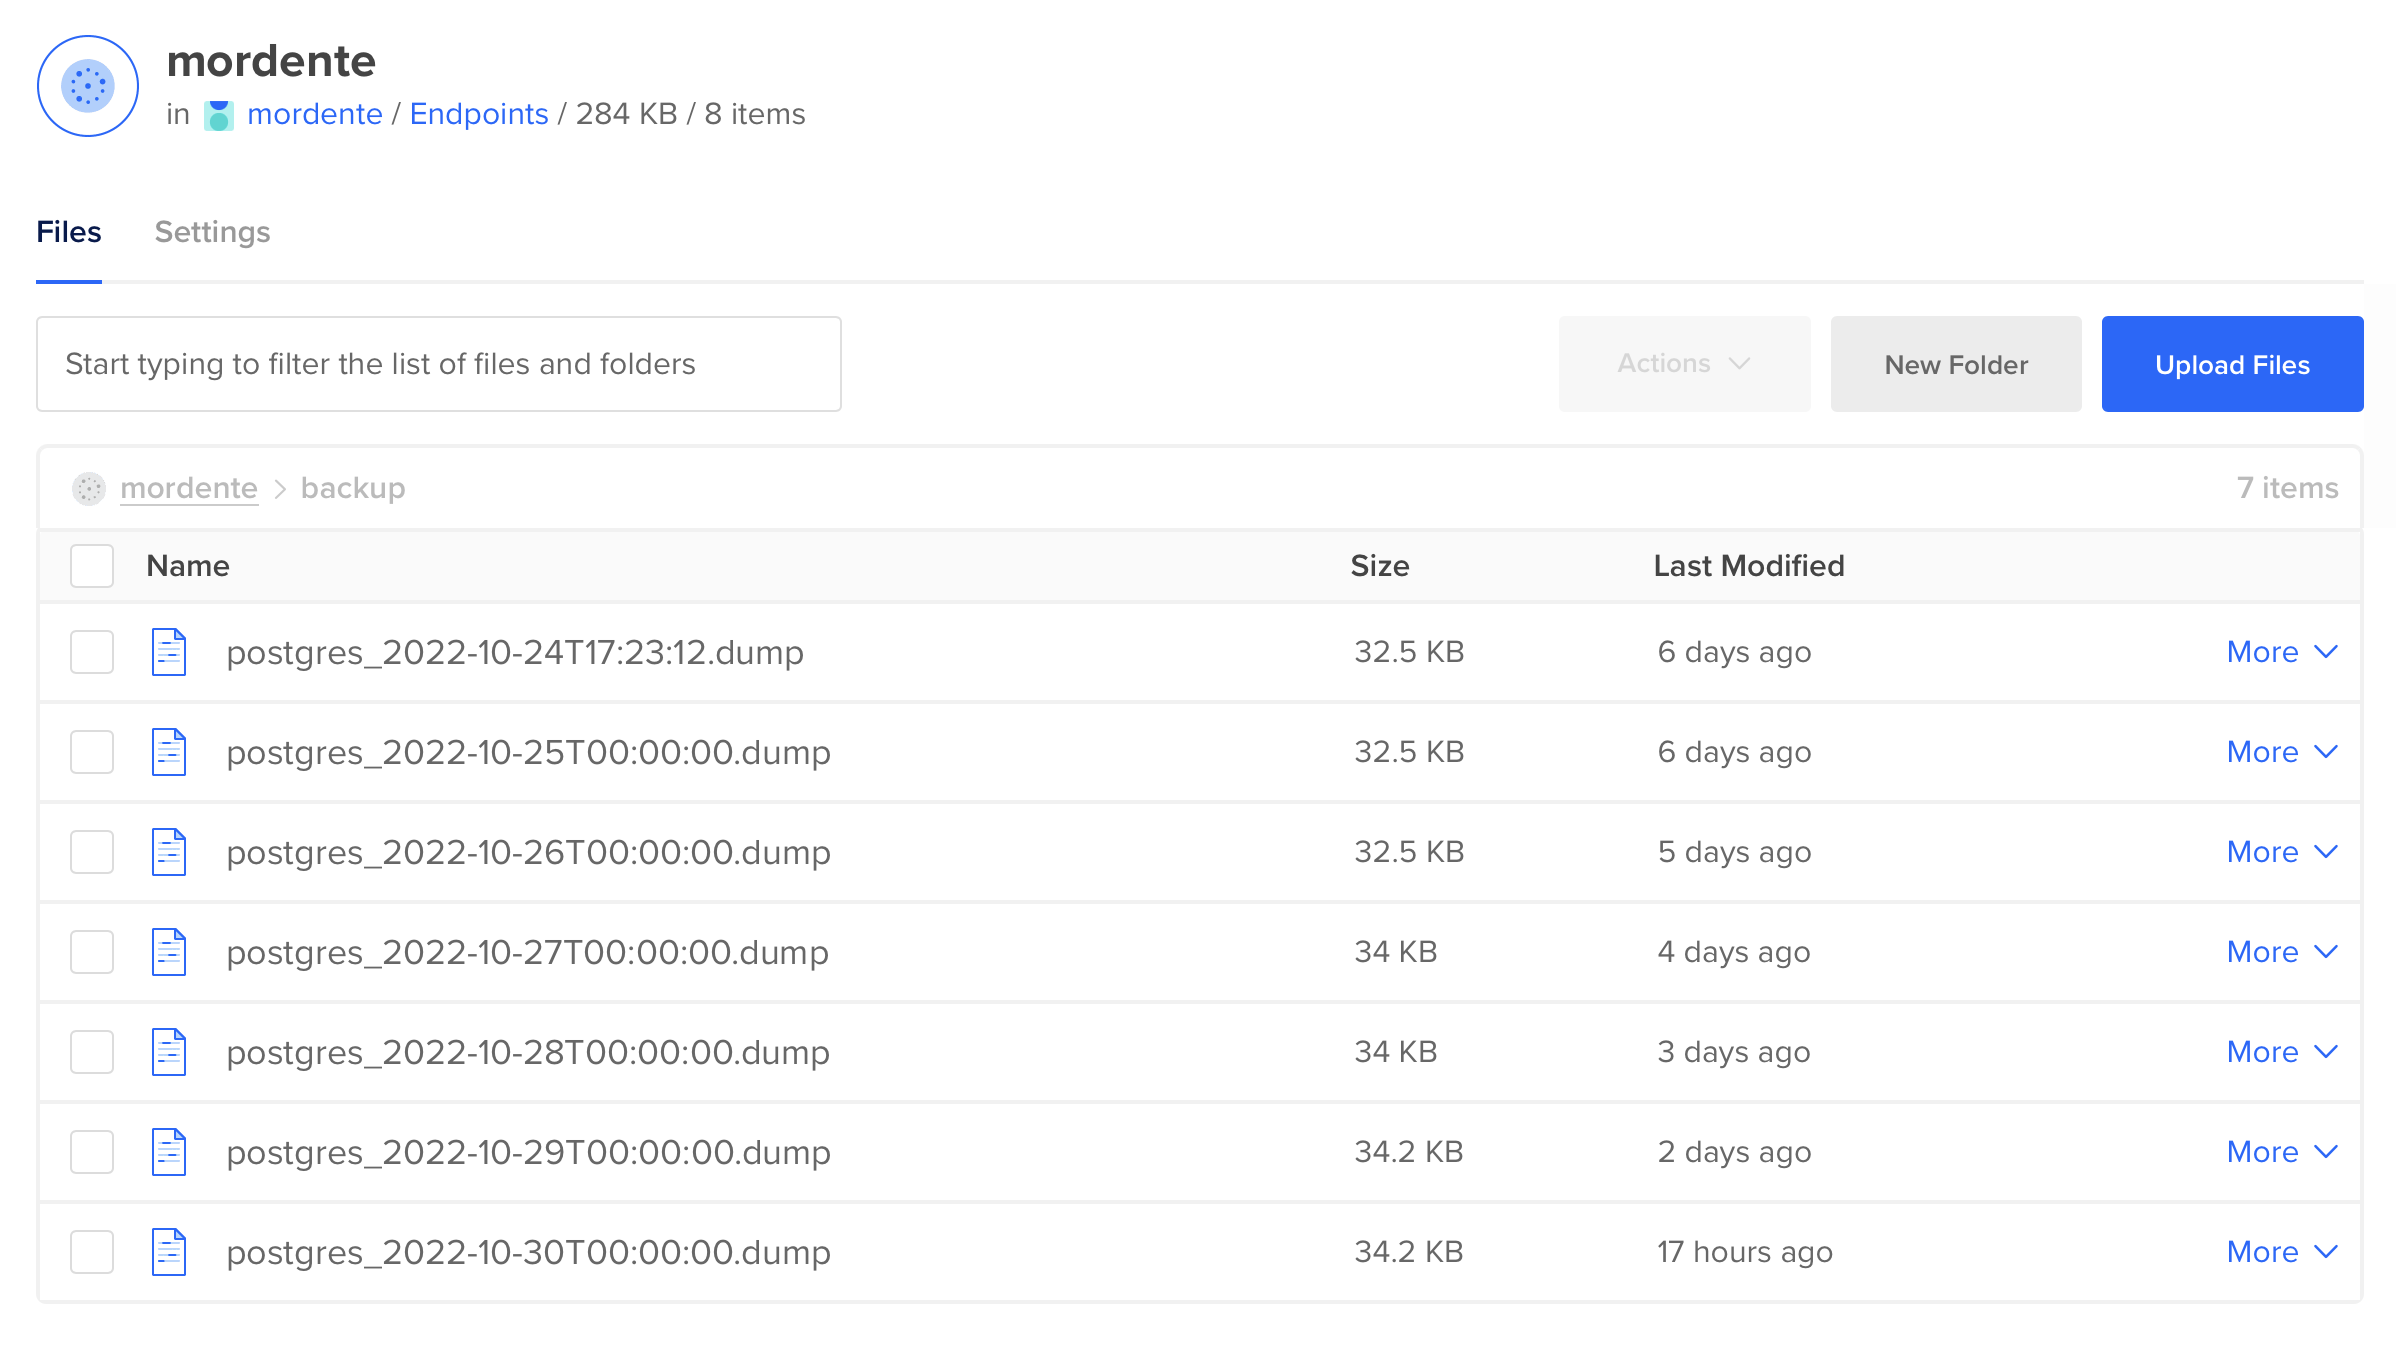
\includegraphics[width=0.75\textwidth]{imagenes/implementacion/backup_antes_de_borrado_automatico.png}
\caption{Archivos en el \textit{bucket S3} antes de superar el máximo de días configurado}
\label{fig:backup1}
\end{figure}

\begin{figure}[h]
\centering
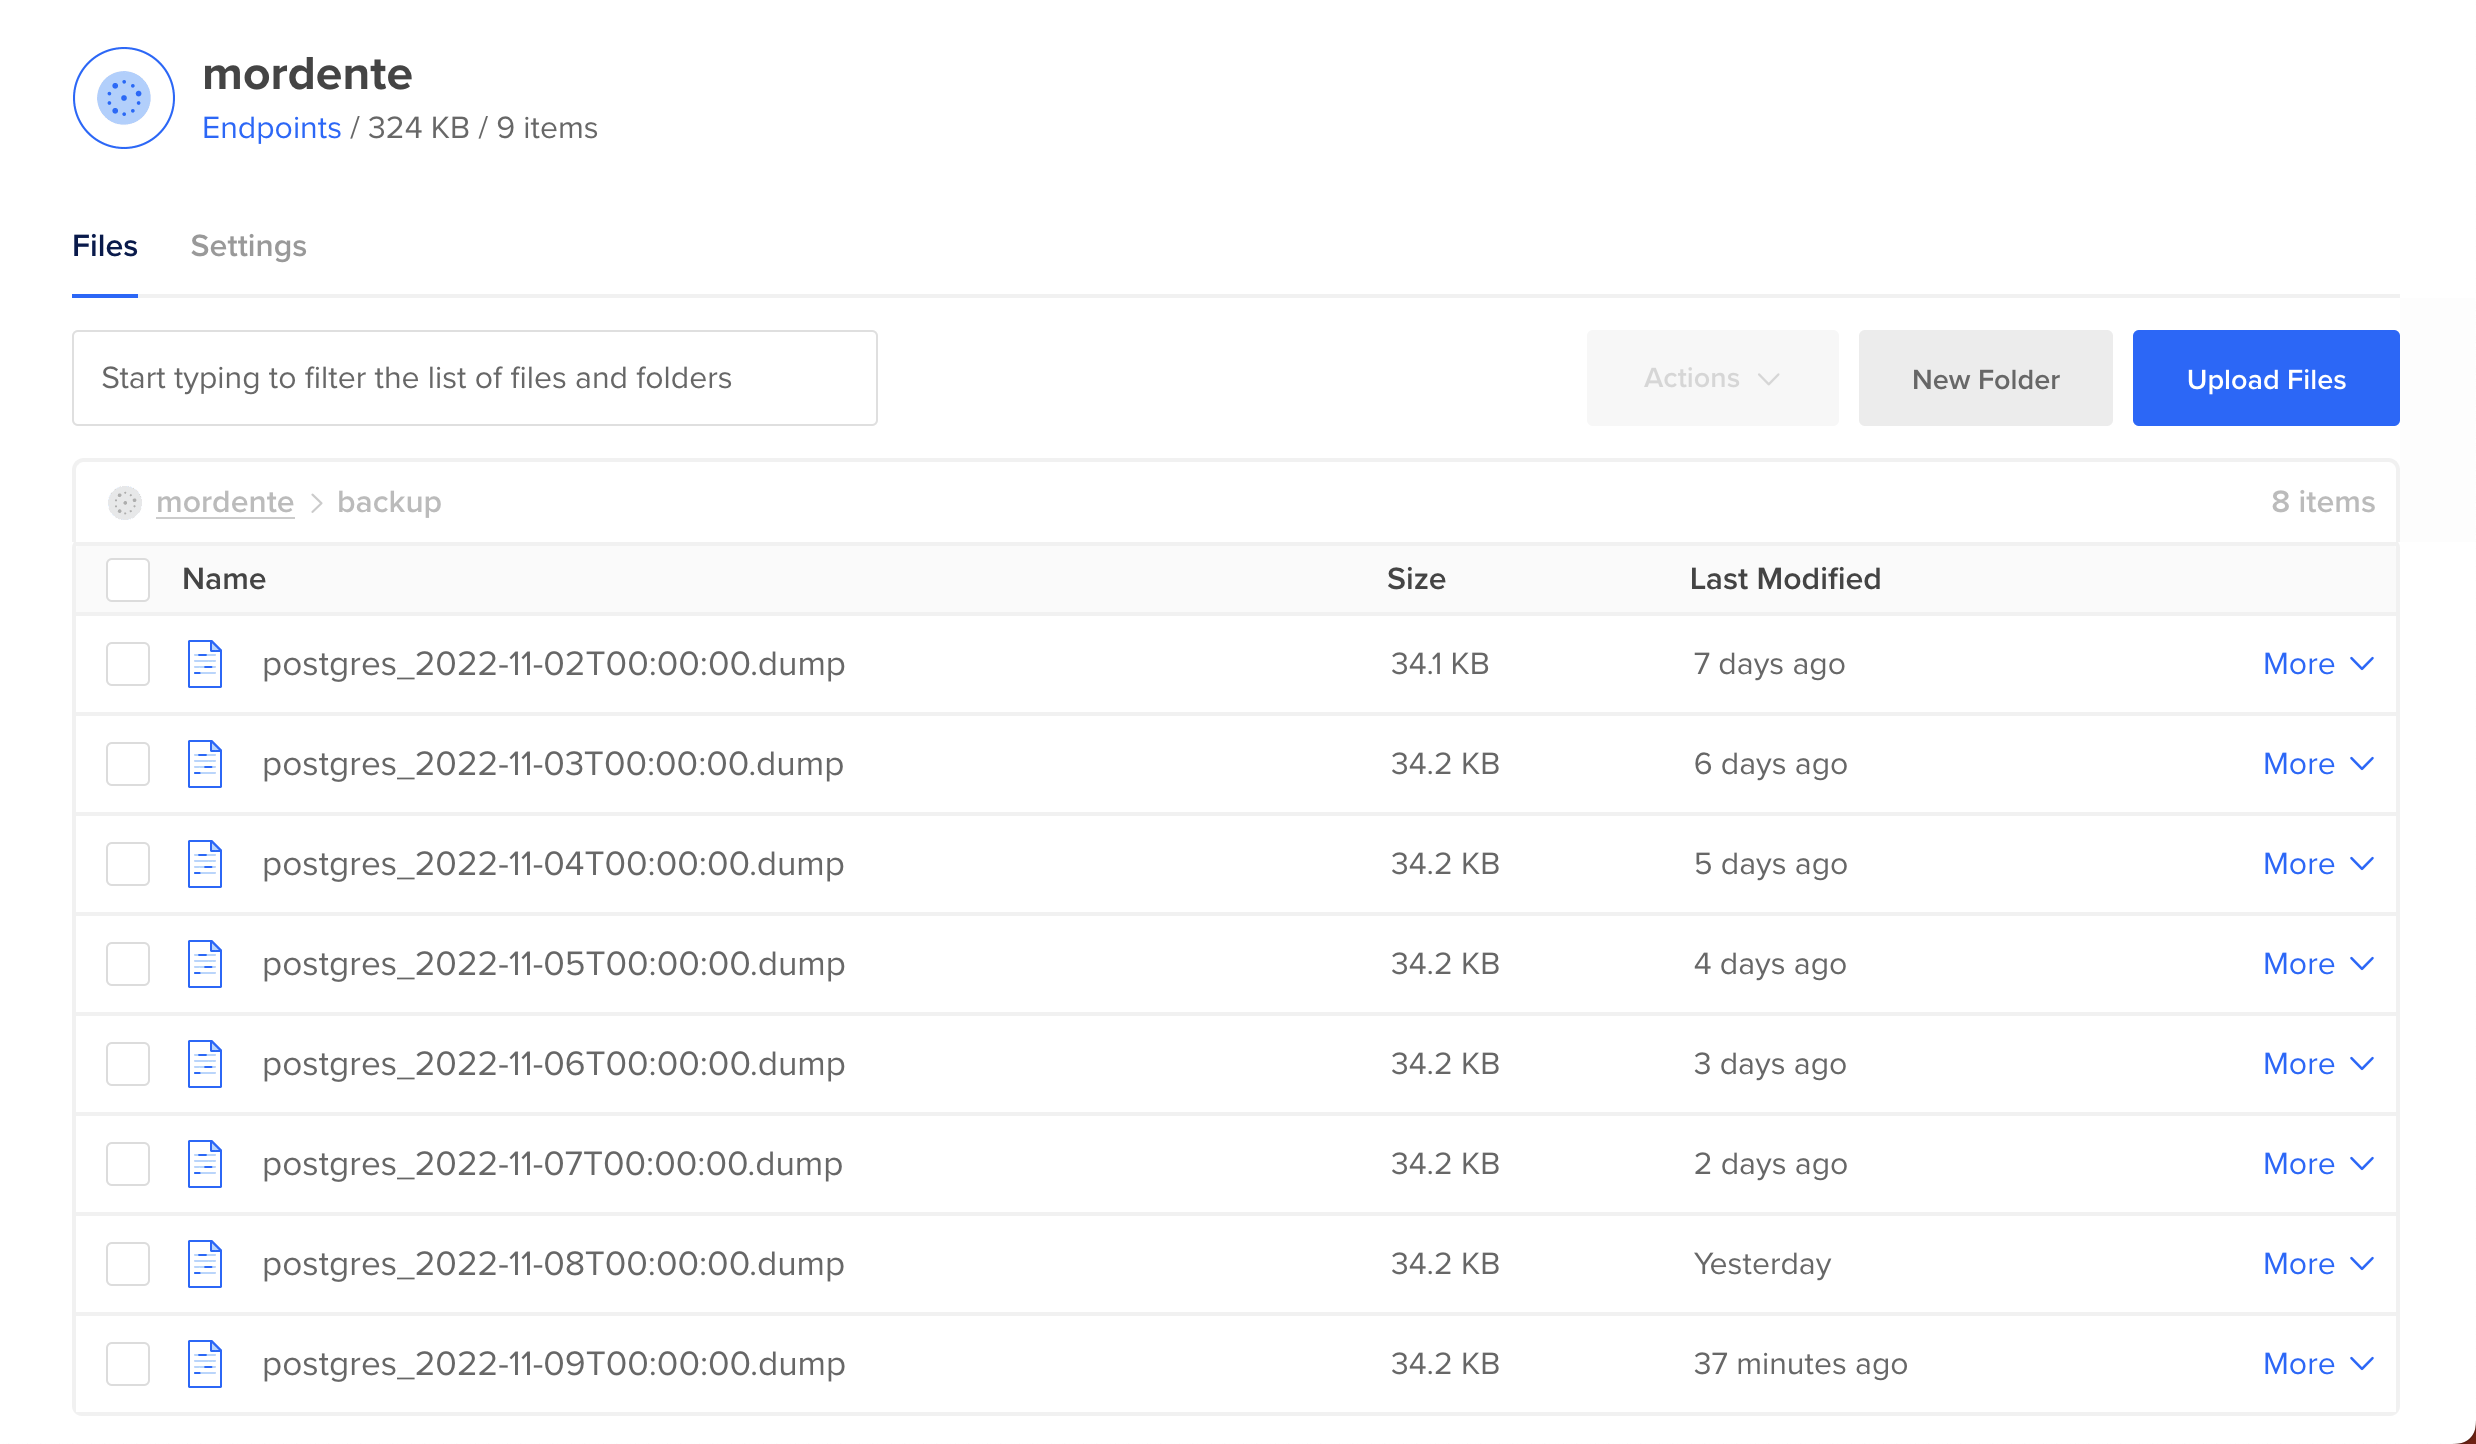
\includegraphics[width=0.75\textwidth]{imagenes/implementacion/backup_despues_borrado_automatico.png}
\caption{Archivos en el \textit{bucket S3} tras superar el máximo de días configurado}
\label{fig:backup2}
\end{figure}




\section{Despliegue Continuo (CD): Automatizando el despliegue del bot a producción}

% https://github.com/daniharo/mordente/commit/8965e0e893ea7ccf87da4947a8ba1ebf462d0c43

% https://github.com/daniharo/mordente/commit/6ade5d3554df9d49b8ece3adc08c54875c597397

Cuando cambiamos el código del proyecto, para actualizar el código que tenemos subido en el servidor de producción tenemos que seguir los siguientes pasos:

\begin{enumerate}
    \item Acceder mediante \texttt{ssh} al servidor.
    \item Actualizar el código con \texttt{git pull}.
    \item Reconstruir la imagen de \texttt{docker} usando el comando \texttt{docker compose up --build}.
\end{enumerate}

Dado que estos pasos se van a seguir de formar repetitiva cada vez que 

Es aquí cuando entra en juego el \textbf{Despliegue Continuo (CD)}: es una técnica que consiste en desplegar automáticamente la aplicación a producción cuando se realizan cambios (\textit{commits}) en el código\cite{Shahin_2017}. 
% https://arxiv.org/pdf/1703.07019.pdf

\textbf{GitHub} permite emplear esta técnica fácilmente mediante el uso de las llamadas \textbf{Github Actions}\footnote{\url{https://github.com/features/actions}}: mediante el añadido de ciertos archivos especiales al repositorio, \textbf{GitHub} ejecuta las acciones especificadas en los supuestos que configuremos.

En nuestro caso, queremos que cuando haya nuevo código en \textit{GitHub} para la rama \texttt{main} se ejecuten automáticamente los pasos reseñados en el comienzo de esta sección. Para ello, añadimos un archivo en la ruta \path{.github/workflows/deploy.yml}, en el cual especificamos cuándo queremos que se ejecute (en los \texttt{git push} a \texttt{main}), qué pasos hay que seguir, además de otras configuraciones que se pueden ver en el \textit{commit} correspondiente\footnote{\url{https://github.com/daniharo/mordente/commit/8965e0e8}}.

A partir de este momento, tal y como se puede ver en la figura \ref{fig:marcaDeploy}, a la derecha de cada \textit{commit} en \textbf{GitHub} aparece un símbolo a modo de marca de verificación en color verde, indicando que el despliegue se ha completado sin problemas. Al hacer clic aparece un botón de \textbf{Detalles} que nos permite consultar cómo se ha llevado a cabo el despliegue\footnote{Ejemplo: \url{https://github.com/daniharo/mordente/actions/runs/3416143998/jobs/5685987409}}.

Los datos para el acceso mediante \texttt{ssh} al servidor se almacenan cifrados como \texttt{Environment secrets}\footnote{\url{https://docs.github.com/en/actions/security-guides/encrypted-secrets}}, de modo que en ningún momento nadie más que el creador del proyecto tiene acceso a ellos. Además, solo los usuarios con permisos de escritura en la rama \texttt{main} pueden disparar un nuevo despliegue.


\begin{figure}[h]
\centering
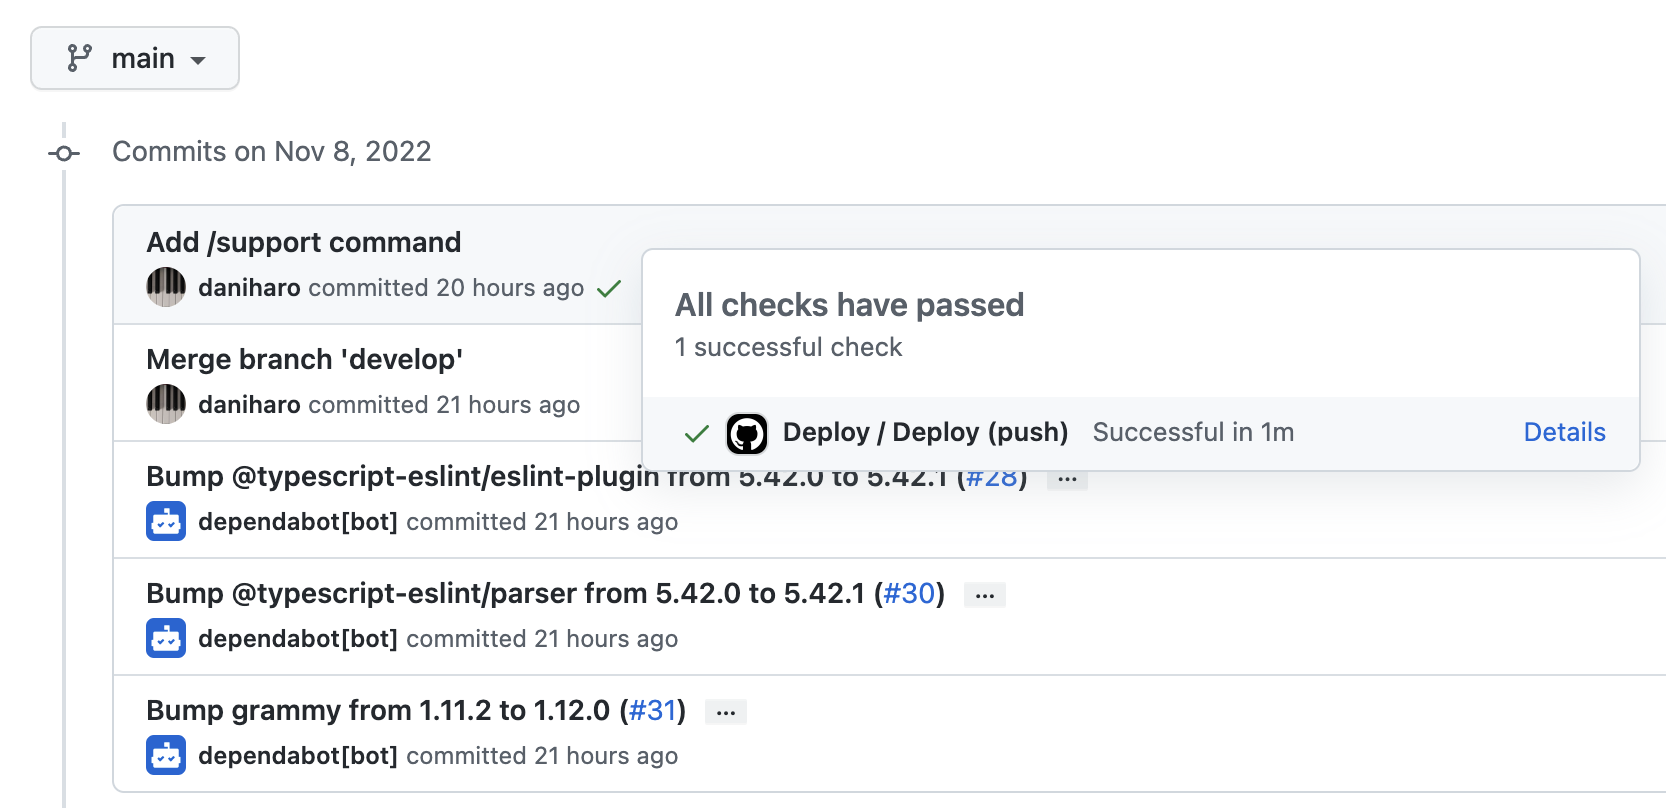
\includegraphics[width=0.75\textwidth]{imagenes/implementacion/marcaDeploy.png}
\caption{Marca de verificación del \textbf{Despliegue Continuo}}
\label{fig:marcaDeploy}
\end{figure}

Más tarde se ha implementado una configuración para que al modificar ciertos archivos como el \texttt{README.md} no se provoque un despliegue\footnote{\url{https://github.com/daniharo/mordente/commit/6ade5d35}}.


\section{Configurando la detección automática de vulnerabilidades}

% https://github.com/daniharo/mordente/commit/87541359abe2dc01ab819241ef8b595d729d21e7

Se ha detectado que una tarea frecuente durante el desarrollo de este proyecto ha sido revisar periódicamente de forma manual si alguna de las dependencias\footnote{Las dependencias del bot se especifican en el archivo \texttt{package.json}: \url{https://github.com/daniharo/mordente/blob/main/package.json}} usadas ha sido actualizada por haberse detectado alguna vulnerabilidad o por incorporar nuevas funcionalidades.

Es por ello que se ha configurado una herramienta automática que comprueba diariamente las dependencias y crea un \textit{Pull Request} para cada actualización. Esta herramienta la proporciona \textit{GitHub}, y su nombre es \textit{Dependabot}.

Para configurarla se ha añadido un archivo en la ruta \path{/.github/dependabot.yml}\footnote{\url{https://github.com/daniharo/mordente/commit/8754135}} especificando el intervalo entre detecciones (en nuestro caso cada día o \texttt{daily}), la ruta donde se encuentra el \texttt{package.json} con las dependencias y en qué rama queremos que se hagan los \textit{Pull Request} (\texttt{develop} ya que \textit{main} es la rama de producción).

Una vez configurado, comprobamos que cuando hay actualizaciones disponibles obtenemos las notificaciones correspondientes indicándolo\footnote{Ejemplo: \url{https://github.com/daniharo/mordente/pull/25}}.

\section{La función de editar}
% https://github.com/daniharo/mordente/commit/3e630b1fe45c479f836f21de003e7f6cc7f0bbee

La última funcionalidad que falta para que el bot sea usable es la de \textbf{editar} elementos, ya sean agrupaciones, eventos u obras. 

Dado que el tiempo restante para terminar el proyecto es limitado, se ha decidido implementar solo la edición de agrupaciones de forma que la edición de eventos y obras estaría preparada, solo pendiente de readaptar el código ya implementado.

El flujo del usuario será:
\begin{enumerate}
    \item Abrir el detalle de la agrupación.
    \item Pulsar el botón de ``Editar'' debajo del detalle, que solo aparecerá si es usuario administrador.
    \item Seleccionar en el menú qué atributo quiere editar.
    \item Responder al bot con el nuevo valor.
    \item Finalmente el usuario recibe una confirmación de que la agrupación ha sido modificada con éxito.
\end{enumerate}

\sloppy
Para ello, implementamos el menú para seleccionar qué atributo vamos a editar (\texttt{editEnsembleMenu}) y una nueva conversación para cada atributo que se puede editar: \texttt{editEnsembleNameConversation}, \texttt{editEnsembleDescriptionConversation}...

Los cambios en el código se pueden ver en el repositorio\footnote{\url{https://github.com/daniharo/mordente/commit/3e630b1}}.


\section{Página web: \href{https://mordente.es}{\texttt{mordente.es}}}

Una vez tenemos la aplicación funcionando y lista para poder hacer pruebas con usuarios, es conveniente desarrollar un sitio web donde explicar qué es Mordente, qué hace y cómo funciona. En esta sección se va a describir el proceso que se ha seguido para conseguirlo.

\subsection{Creación del proyecto}

Como venimos haciendo a lo largo del proyecto, hemos creado un repositorio público vacío en GitHub con el nombre de \texttt{mordente-docs}\footnote{\url{https://github.com/daniharo/mordente-docs}}. Seguidamente se ha clonado en el equipo de desarrollo usando el siguiente comando de \texttt{git}:

\begin{verbatim}
git clone git@github.com:daniharo/mordente-docs.git
\end{verbatim}

En la sección \ref{subsection:decisionDocumentacion} se ha decidido usar la herramienta \texttt{docusaurus} para desarrollar la página web, por lo tanto seguiremos sus instrucciones\footnote{\url{https://docusaurus.io/docs/installation}} para iniciar el desarrollo. Tras seguir las instrucciones, ya tenemos la estructura preparada para crear el contenido\footnote{\url{https://github.com/daniharo/mordente-docs/commit/1c25316}}.

\subsection{Creación de contenido}

La estructura de código que nos proporciona \texttt{docusaurus} nos permite configurar la estructura, apariencia y contenido de la página web partiendo de una plantilla \textit{responsive} (adaptada a todos los tamaños de pantalla) y accesible.

Aprovecharemos las posibilidades de configuración que nos ofrece \texttt{docusaurus} para cambiar los colores a nuestra paleta, añadir el logotipo y el contenido personalizado.

Algunas de las herramientas usadas durante este paso han sido:
\begin{itemize}
    \item \texttt{undraw}\footnote{\url{https://undraw.co/}}: es una extendsa biblioteca de ilustraciones SVG a las cuales se les puede personalizar fácilmente el color, y que representan distintas situaciones o ideas.
    \item \texttt{favicon-generator}\footnote{\url{https://www.favicon-generator.org/}}: el \texttt{favicon} es el icono que aparece a la izquierda del título de la página en el navegador. El archivo debe ubicarse en la raíz del directorio de la página y llamarse \texttt{favicon.ico}. Esta herramienta nos permite convertir cualquier imagen a un \texttt{favicon} con la medida adecuada.
    \item Se han usado algunos conocimientos previos de \texttt{react}\footnote{\url{https://reactjs.org/}}, ya que \texttt{docusaurus} está basado en esta biblioteca de interfaces de usuario.
\end{itemize}

En GitHub se pueden observar los cambios exactos realizados en el código para añadir el contenido de la página web\footnote{\url{https://github.com/daniharo/mordente-docs/compare/fd28973...e8980b0}}.



\subsection{Alojar en servidor}

Para que la página web esté accesible públicamente, es necesario alojarla en un servidor público. Existen múltiples plataformas que permiten alojar fácilmente contenido estático\footnote{Con \textit{contenido estático} nos referimos a archivos \texttt{HTML}, \texttt{CSS}, imágenes, etc. que se envían directamente al cliente sin necesidad de que haya una lógica en el servidor para calcularlos.} como el que genera \texttt{docusaurus}, pero las más interesantes permiten actualizar automáticamente el contenido del servidor cada vez que hay un \texttt{commit} en la rama principal del repositorio. Algunas de las más conocidas son:

\begin{itemize}
    \item \textbf{Vercel}\footnote{\url{https://vercel.com/}}: Es la empresa que desarrolla el \textit{framework} \texttt{Next.js}, una de las herramientas más usadas\footnote{\url{https://survey.stackoverflow.co/2022/\#most-popular-technologies-webframe}} por su flexibilidad para crear páginas web requieran de lógica en el servidor o no. Su servicio de alojamiento de páginas web destaca por su facilidad de uso, con una configuración automática e inmediata.
    \item \textbf{Netlify}\footnote{\url{https://www.netlify.com/}}: Principal competidor de Vercel, ofrece más posibilidades de configuración pero un peor rendimiento.
    \item \textbf{Github Pages}\footnote{\url{https://pages.github.com/}}: Es un servicio prestado por la forja de repositorios \textbf{GitHub}. Requiere de una configuración más compliacada para automatizar la compilación del código\footnote{\url{https://docusaurus.io/docs/deployment\#deploying-to-github-pages}}.
    \item \textbf{Cloudflare Pages}\footnote{\url{https://pages.cloudflare.com/}}: Nuevo servicio equivalente a Netlify o Vercel, con una configuración igual de sencilla. Es provisto por Cloudflare, una compañía especializada en prestar servicios de \textit{caché de contenido} y de seguridad.
\end{itemize}

Se optará por \textbf{Vercel} por la familiaridad del desarrollador de este proyecto con este proveedor por proyectos anteriores y por su facilidad de uso.

Para alojar nuestra página en \textbf{Vercel}, simplemente seguimos la documentación\footnote{\url{https://docusaurus.io/docs/deployment\#deploying-to-vercel}}, tarea que no nos lleva más de unos minutos. Una vez hemos terminado, tenemos la página web en una dirección asignada automáticamente: \url{https://mordente.vercel.app}.

\subsection{Redirecciones}

Para facilitar el acceso al contenido de este trabajo, se va a configurar el servidor de manera que al acceder a ciertas rutas se abra una determinada página de un dominio externo. Lo haremos siguiendo las instrucciones de Vercel para ello\footnote{\url{https://vercel.com/docs/project-configuration\#project-configuration/redirects}}. Las rutas que redireccionaremos están descritas en la tabla \ref{tab:redirecciones}.

\begin{table}[]
    \centering
    \begin{tabular}{|l|c|}
        \hline
        \textbf{Ruta origen} & \textbf{Redirige permanentemente a} \\
        \hline
        \href{https://mordente.es/repo}{\texttt{/repo}} & \multirow{2}{*}{Código del bot} \\ \cline{1-1}
        \href{https://mordente.es/source}{\texttt{/source}} & \\ \hline
        \href{https://mordente.es/source/docs}{\texttt{/source/docs}} & Código de la página web \\
        \hline
        \href{https://mordente.es/source/memoria}{\texttt{/source/memoria}} & Código \LaTeX{} de la memoria \\
        \hline
        \href{https://mordente.es/memoria}{\texttt{/memoria}} & Memoria en formato \texttt{PDF} \\
        \hline
        \href{https://mordente.es/try}{\texttt{/try}} & Bot en Telegram \\
        \hline
    \end{tabular}
    \caption{Redirecciones en \href{https://mordente.es}{\texttt{mordente.es}}}
    \label{tab:redirecciones}
\end{table}

\subsection{Asignación de dominio}\label{subsection:asignacionDominio}

Registrar un dominio personalizado nos permitirá acceder a la página con una dirección sencilla y fácil de recordar. 

Las empresas encargadas de registrar un dominio son llamadas \textbf{registradores de dominios}. Tras comparar precios entre diversos registradores para dominios \texttt{.es}, en nuestro caso se opta por \textbf{IONOS}\footnote{\url{https://www.ionos.es/dominios/}}, que ofrece el dominio \texttt{mordente.es} por 1,21\texteuro{} el primer año, la mejor oferta entre las encontradas.

Tras hacer el proceso de compra, seguimos las instrucciones\footnote{\url{https://vercel.com/docs/concepts/projects/domains/add-a-domain}} de \textbf{Vercel} para asignar el dominio al proyecto. Esperamos un tiempo aproximado de una hora mientras se propagan los nuevos registros DNS, tras el cual Vercel genera automáticamente el certificado TLS para nuestro dominio\footnote{\url{https://vercel.com/blog/automatic-ssl-with-vercel-lets-encrypt}} y podemos acceder sin problemas a \url{https://mordente.es}.

El último paso es modificar la configuración de \texttt{docusaurus} para ajustar correctamente el nuevo dominio principal\footnote{\url{https://github.com/daniharo/mordente-docs/commit/c2e2f8e}}.

\subsection{Probando otros proveedores}

Durante la realización de un proyecto personal paralelo\footnote{Aplicación usando ingeniería inversa para consultar en tiempo real los tiempos de paso del Metropolitano de Granada: \url{https://metrogranada.pages.dev}. Código en \url{https://github.com/daniharo/Metro-Granada-Webapp}.} se ha comprobado cómo \textbf{Cloudflare Pages}, siendo un proveedor muy parecido a \textbf{Vercel}, proporciona un menor tiempo de respuesta (aproximadamente la mitad) a la hora de alojar un servidor \texttt{Next.js}\footnote{\url{https://nextjs.org/}} que incluye \textit{Rutas API Edge}\footnote{\url{https://nextjs.org/docs/api-routes/edge-api-routes}}.


Es por esto que se ha querido comprobar si para sitios puramente estáticos como el que hemos creado en esta sección, \textbf{Cloudflare Pages} es capaz también de dar un mayor rendimiento.

Para ello, se han seguido las instrucciones correspondientes, primero para alojar el contenido \footnote{\url{https://developers.cloudflare.com/pages/framework-guides/deploy-a-docusaurus-site/}} y después para asignar el dominio que creamos en la sección \ref{subsection:asignacionDominio}\footnote{\url{https://developers.cloudflare.com/pages/platform/custom-domains/}}. Por último se han añadido las redirecciones en el formato requerido por Cloudflare\footnote{\url{https://developers.cloudflare.com/pages/platform/redirects/}} (y que coincide con \textbf{Netlify}\footnote{\url{https://docs.netlify.com/routing/redirects/}}).


\subsubsection{Conclusiones del cambio de proveedor}

Tras seguir las instrucciones, hemos podido comprobar que aunque por culpa de una configuración por defecto incorrecta\footnote{\url{https://stackoverflow.com/a/74341851/12210701}} parecía que habíamos empeorado el rendimiento, tras solucionar la configuración sí que se ha mejorado el tiempo de respuesta con respecto a Vercel, aunque en una proporción despreciable (unos 120ms en Cloudflare frente a 140ms en Vercel).

Sin embargo, estas mediciones se hicieron por la noche, mientras la mayoría mediciones hechas durante el día indican que \textbf{Cloudflare} necesita un mayor tiempo para entregar la web: unos 250ms, frente a 140ms en Vercel.

Se ha detectado que el motivo es que, para reducir la carga de algunos centros de datos, algunas peticiones a páginas que están en el plan gratuito se enrutan a centros de datos lejanos\footnote{\url{https://community.cloudflare.com/t/peering-why-dont-i-reach-the-closest-datacenter-to-me/76479}}. En nuestro caso, hemos visto peticiones dirigidas a centros de datos en India o Estados Unidos, mientras que \textbf{Vercel} enruta todas las peticiones a Frankfurt (Alemania).

Es por esto que se ha decidido revertir el cambio de proveedor.


\section{Creación de dirección de email}

El proveedor de DNS utilizado para \texttt{mordente.es} nos permite obtener una dirección de correo electrónico gratuita con 2GB de almacenamiento. Por tanto, se ha creado una dirección 
de soporte (\texttt{soporte@mordente.es}) para los usuarios que puedan tener alguna consulta.

% cuatrimestre 15 semanas